%%%%%%%%%%%%%%%%%%%%%%%%%%%%%%%%%%%%%%%%
%   Original by                                   %
% Athanassios Protopapas, October 2005 %
% Mini-example for using apa.cls       %
%                                      %
% modified by William Revelle, August, 2007 
%%%%%%%%%%%%%%%%%%%%%%%%%%%%%%%%%%%%%%%%

\documentclass[man]{apa}%can be jou (for journal), man (manuscript) or doc (document)
%
%
%these next packages extend the apa class to allow for including statistical and graphic commands
\usepackage{url}   %this allows us to cite URLs in the text
\usepackage{graphicx}  %allows for graphic to float when doing jou or doc style
\usepackage{amssymb}  %use formatting tools  for math symbols
% type setting of functions, packages, and R follows a particular style


\usepackage{multicol}
\usepackage{setspace}



\title{Are divergence point analyses suitable for latency data?}
\author{Pablo Gomez (1), Javier Breithaupt (2), Manuel Perea(2, 3), Jeff Rouder (4)}
\affiliation{(1) DePaul University, Chicago, USA \\ 
                 (2) Universitat de Val\`encia, Val\`encia, Spain \\ 
                 (3) BCBL, Basque Center on Cognition, Brain, and Language, San Sebasti\'a�n, Spain \\
                 (4) University of Missouri}
%taken from AP's user notes
% John Vokey uses something like this

\ifapamodeman{%

\note{\begin{flushleft}
Pablo Gomez\\
Department of Psychology\\
DePaul University\\
Chicago, Illinois\\
60614\\
e-mail: pgomez1@depaul.edu\\

   
\end{flushleft}}}


\abstract{
The uncovering of the time course of the influence of different factors in human performance is one of the principal topics of research in cognitive psychology/neuroscience. Over the past decades, researchers have proposed several methods to tackle this question using latency data. Here we examined a recently proposed procedure that employs survival analyses on latency data to provide ``precise estimates'' of the timing of the first discernible influence of a given factor on performance (e.g., word frequency on lexical access).  A number of articles have used this method in recent years, and hence an exploration of its strengths and its potential weaknesses is in order. Unfortunately our analysis revealed that the method has fundamental conceptual flaws, and it might lead researchers into believing that they are obtaining a measurement of a processing component when in fact they are obtaining a non-sensical measurement.
}

\acknowledgements{
The research reported in this article has been partially supported by Grant PSI2014-53444-P from the Spanish Ministry of Economy and Competitiveness. Pablo Gomez was the recipient of the``Convitat'' grant at the University of Valencia (VLC-Campus).
}


\shorttitle{Survival and latencies}
\rightheader{Survival and latencies}
\leftheader{Gomez, Breithaupt, Perea \& }

\begin{document}
\maketitle   



Perhaps the most common cognitive psychology experiment is one in which participants are presented with stimuli that vary in a dimension of theoretical interest (e.g., length, word frequency, etc.). The stimulus elicits a response, and researchers often measure latencies to make inferences about hypothesized underlying cognitive processes.  This form of mental chronometry is widely used in the analyses of data from a wide range of experimental paradigms such as choice tasks, naming, eye-tracking, and many others.

   The most popular model of analysis are tests of mean latencies.  The shortcomings of focusing on mean latencies to understand hypothesized processes are well known (Balota \& Yap, 2011; Heathcote, Popiel, \& Mewhort, 1991; Ratcliff, 1979); hence, theory development benefits from exploring distributional properties of latency measurements.  To take advantage of the distributional information, some researchers use methods that are based on fitting functional forms like the ex-Gaussian or the Weibull distributions (see Heathcote et al., 1991), and other researchers use methods that are based on process models like the diffusion model for choice response times (Ratcliff, 1978) or the EZ-reader model for eye fixation durations during reading (Reichle, Pollatsek, Fisher, \& Rayner, 1998). 
           
      Is there a method that goes beyond mean latency analyses without making strong theoretical commitments or specific assumptions about distributional properties of the latency measurements and does not require a specific experimental paradigm?  In this note, we consider a method proposed to fulfill that void in the literature, namely, the \emph{divergence point analysis} (Reingold, Reichle, Glaholt, \& Sheridan, 2012; Sheridan, 2013), which was proposed as a way to estimate the onset of the influence of a given variable (the divergence point) on the basis of latency data (e.g., response times or eye fixation times).  

       Recently, Sheridan, Reingold, and colleagues (Sheridan, 2013; see also Ando, Matsuki, Sheridan, \& Jared, 2015; Reingold \& Sheridan, 2014; Reingold, et al,, 2012; Sheridan \& Reingold, 2013; Sheridan, Rayner \& Reingold, 2013) proposed a method that promises to overcome the limitations of traditional survival function analyses by using a computationally intensive bootstrapping procedure.  This procedure compares the latency distributions of two conditions by estimating the divergence point. The divergence point corresponds to the shortest latency value at which a manipulation has a significant impact. Thus, the divergence point offers an estimate of the timing of the first discernible influence of a given variable (e.g., word frequency in a word recognition task). Furthermore, this method can also inform us whether the effect of a given factor has an earlier onset than the effect of another factor. 
      
         
         Divergent point analysis identifies this onset time as follows:  Let T be a random variable that denotes the response time and let F(t) be its cumulative distribution function (CDF).    CDFs denote the probability that the response occurs less than some value t, i.e., $F(t)=Pr(T<=t)$.  The survival function is the complement probability, $S(t)=Pr(T>t)=1-F(t)$, the probability that a response occurs greater than some value t; hence at $t=0$, $S(0) = 1$ and at $t=\infty$, $S( \infty ) = 0$. There have been attempts to use survival functions in latency analyses.  Notably, Van Zandt (2002) examined several of these procedures and concluded that serious analyses of this type, ``would use samples of at least a few hundred observations" (p. 482). Along similar lines Houpt and Townsend (2010, 2011) discussed a rather sophisticated method of survival analysis that involves experimental methods and a non-trivial algorithm termed survivor interaction contrasts (SIC).

           The basic setup in the \emph{divergence point} method under consideration can be described as follows: In each iteration the latencies for each participant and condition are randomly re-sampled with replacement. These sampled (bootstrapped) latencies are used to compute each participant's survival curves, which in turn are averaged across subjects � \emph{\`a la} Vincentile (Vincent, 1912). Next, for each time bin t the difference between conditions: $\Delta_{t,i}$ are computed ($i^{th}$ iteration from 1 to 10,000), and then sorted. The range between the $5^{th}$ and the $9,995^{th}$ value becomes the confidence interval $CI(\Delta t)$ and the divergence point is defined as the shortest $t$ at which the $CI(\Delta t)$ does not include 0. Aiming for a high temporal resolution, Sheridan and Reingold use $1 ms$ bins (see Figure 1 for an example).%\footnote{We should note that in a recent paper, Reingold and Sheridan (2014) proposed some changes on the original version of the procedure by using confidence intervals rather than point estimates, but the both the conceptual and the technical limitations outlined in the present note apply equally to the original and the modified versions of the procedure.}.
      
\begin{figure}[h] %  figure placement: here, top, bottom, or page
	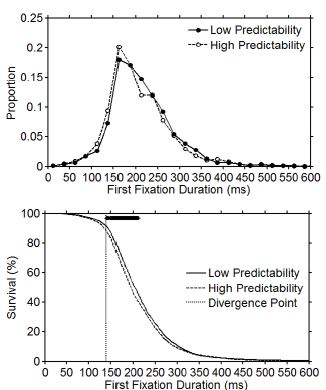
\includegraphics[width=3in]{Figure1.jpg}
    	\label{sheridan}
	\caption{The figure (taken from Sheridan, 2013, page 27) shows the distributions of first-fixation duration on target words in the low and high predictability conditions in the top panel, and the survival curves in the bottom panel. The row of points at the top of the survival curves indicates the time bins with a significant difference between the low and high predictability curves using the method being examined in the present note}
\end{figure}		

      Although this method might seem  promising and useful for researchers interested in exploring the time course of a given  empirical effect, there is a fundamental conceptual flaw in the foundation of the method.

\section{Estimating divergence points in latency distributions is conceptually flawed}

Divergence point analysis rests on the notion that processing in two conditions proceeds in the same way and at the rate until the divergence point.  Then, processing is slowed in one condition relative to the other.  The claim is that by examining the survival functions of RT distributions, the divergence point, should it exist, can be measured.    To show that this claim is flawed, we considered perhaps the simplest case.  Suppose processing was mediated by two stages which operated in serial.  The finishing time of the first stage is a normal with mean $\mu$ and standard deviation $\sigma$; the finishing time of the second stage is an exponential with scale $\tau$.  The manipulation of interest is assumed to affect only the later exponential stage, and it corresponds to a lengthening of scale $\tau$.   In this setup a divergence point might be expected, perhaps at $\mu$.  Figure~\ref{x} shows the density, CDF, and survivor functions for the two cases.  Perhaps counterintuitively, the CDFs have no common points to diverge from.  Instead, the distribution with the smaller exponential scale is faster everywhere.  The relationship is one of strict stochastic dominance.   If one is to talk about a divergence point at all, it would be at  $-\infty.$  

What happens when the divergence-point analysis is applied to this case?  Well the algorithm guarantees a real-valued answer so long as the distributions differ somewhere (and they do here).   In small sample sizes, the smaller differences at the bottom of the distribution cannot be detected and divergence points in the middle of the distribution might be expected.  But in larger sample sizes, the estimate will shift radically downward.  In the large sample limit, the estimate will shift downward without bound.  

This flaw in divergence analysis is easy to understand as a an error in logic.  The claim is based on a moment-to-moment view of processing on a single trial.  Yet, RT distributions are the collection of several trials, and the properties of the distribution do not reflect the properties on any trial.  The flaw is an example of distortions from aggregation which has been well known since Estes (1956).   As an exercise we attempted to think of processing architectures that could yield a true divergence point in the middle of an RT distribution as shown in Figure XXX.  We considered diffusion models, counter models, race models, additive factor and stage insertion models.  These models all fail to produce a true divergence point.  In all cases, there is stochastic dominance, meaning that the divergence happens at the bottom or minimum of the distributions.  We were able to specify one case, a mixture model where the components do not overlap at all.  Such a model is highly artificial and unrealistic in any setting.  It remains an open challenge, one that we suspect cannot be met, to find a plausible process model that predicts a non-minima divergence point.

      
% \begin{figure}[h] %  figure placement: here, top, bottom, or page
%	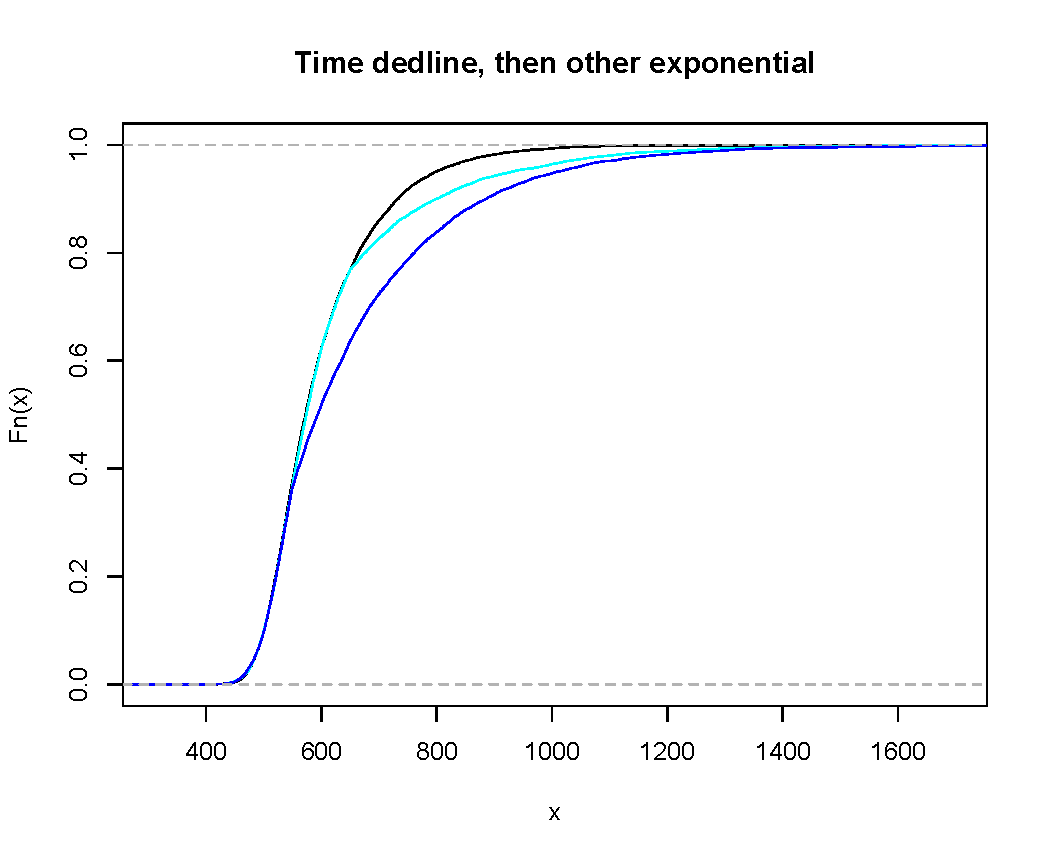
\includegraphics[width=3in]{Figure4.pdf}
%	\label{fig:time}
%	\caption{The figure shows the cumulative density functions generated with two sequential non-cascade processes}
% \end{figure}

\begin{figure}[p] %  figure placement: here, top, bottom, or page
	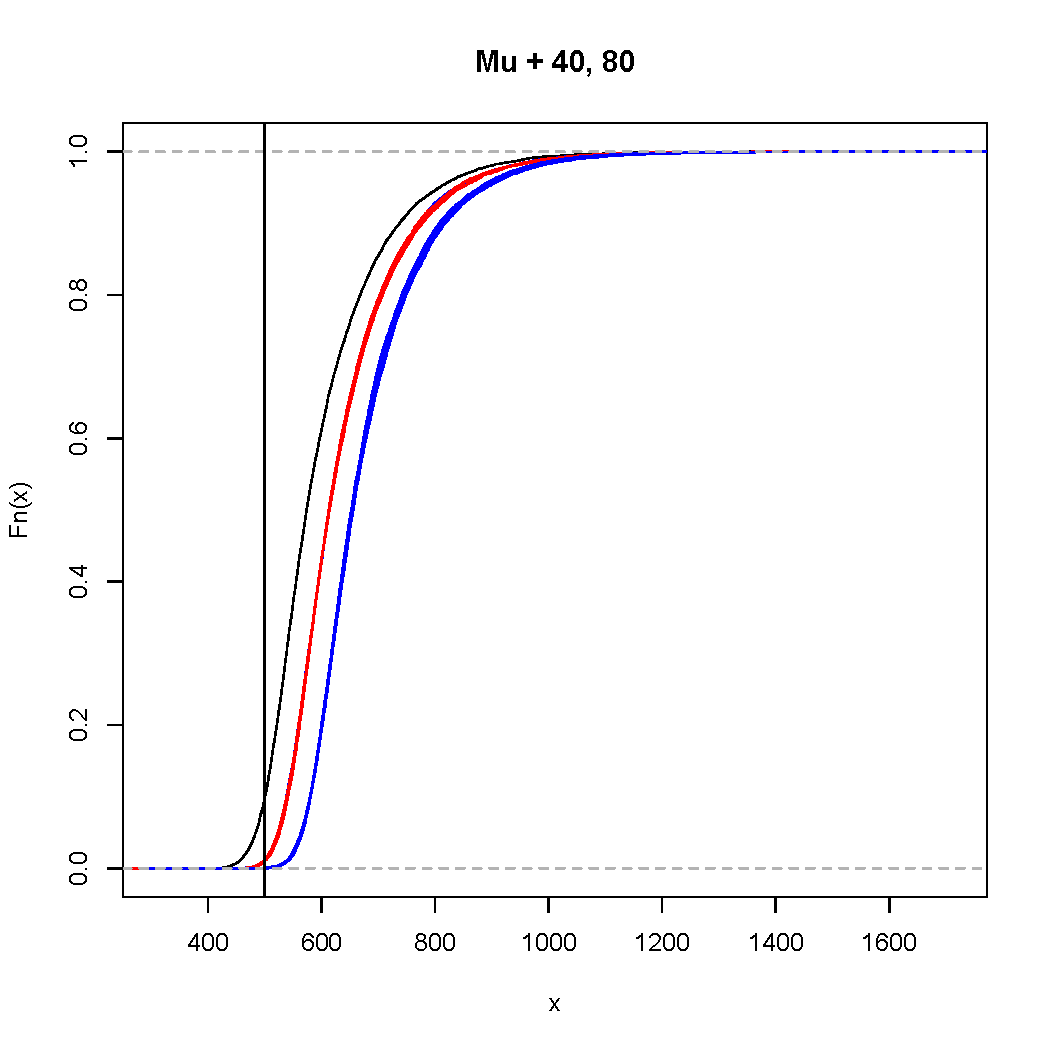
\includegraphics[width=3in]{Figure2.pdf}
   	\label{fig:mu}
	\caption{The figure shows the cumulative density functions generated with an ex-Gaussian distribution in which there are effects on $\mu$}
\end{figure}		


\begin{figure}[h] %  figure placement: here, top, bottom, or page
	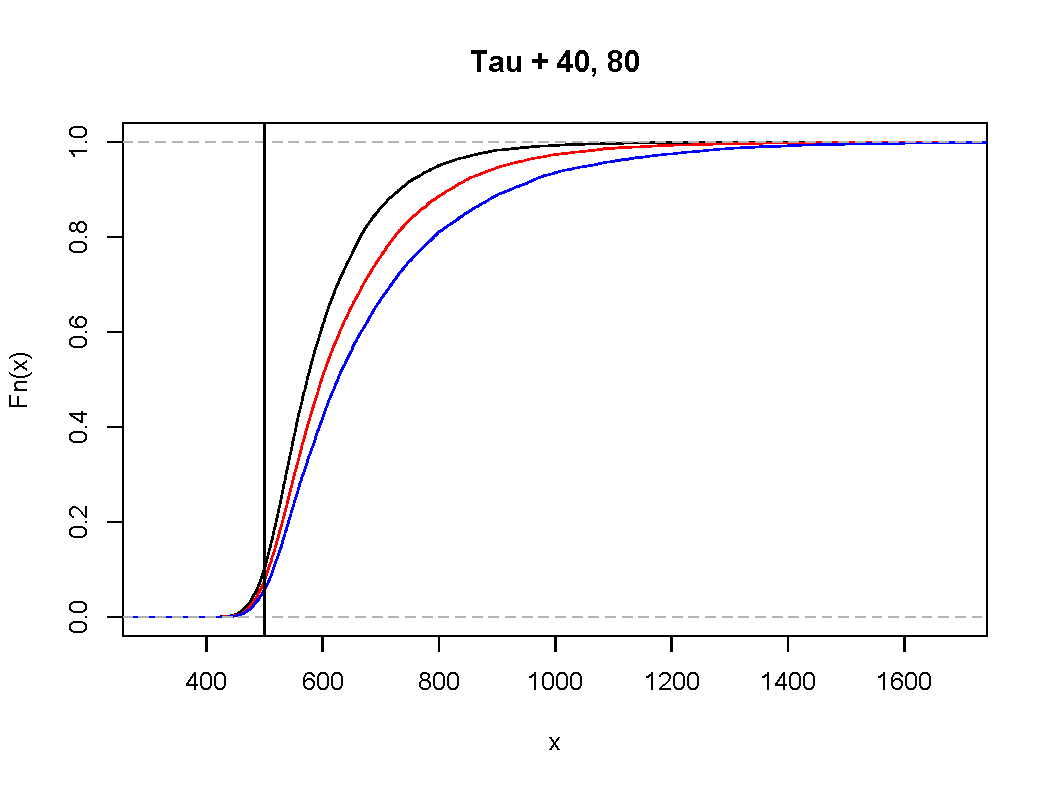
\includegraphics[width=3in]{Figure3.pdf}
	\label{fig:tau}
	\caption{The figure shows the cumulative density functions generated with an ex-Gaussian distribution in which there are effects on $\tau$}
\end{figure}

  
 
  
  \section{The method provides non-sensical results}

      
        What are the consequences of applying this method to data in which there is stochastic dominance? To answer this question, we carried out a series of Monte Carlo simulations. In particular, we generated data from an ex-Gaussian distribution assuming that the experimental effect was either in the $\mu$ or $\tau$ parameters.  We manipulated the number of hypothetical trials per condition and then applied the bootstrapping method to estimate the divergence point.

   For the first simulation, we explored if the method yields false positives when samples are generated from an ex-Gaussian with parameters $\mu= 541$, $\sigma = 68$, and $\tau = 115$ (i.e., a null effect in which identical parameters generate the simulated data for the two conditions; note that these parameters were the average parameters in Heathcote et al, 1991).   The results from this simulation were satisfactory:  The method generates false divergence points less than .01\% regardless of the number of items in the simulations.
   
      In the second simulation, we generated data in which the difference between the two conditions was an effect on $\mu$.  The data for the baseline condition was generated from an ex-Gaussian distribution with $\mu= 541$, $\sigma = 68$, and $\tau = 115$ . We generated data for three simulated experimental conditions by changing $\mu$ to 561, 581 and 621  ($\Delta \mu = 20, 40, 80$) There is, therefore, stochastic dominance of the baseline condition relatively to all of these other conditions, and the true divergence point is at the starting point of the distributions.  The results from this simulation are not encouraging for the method, as the estimation of the divergence point is highly biased by the number of trials per condition ($n = 20, 30, 50, 100, 250, 500, 1000$).   Figure  5 shows the average divergence point for each of the parameter combinations ($\mu$ and $n$) across 1000 simulations. As a consequence of increased statistical power due to larger sample size at the trial level, the larger the number of trials per condition, the shorter the estimated divergence point (i.e., there is a statistical bias dependent on sample size). For example, with $\Delta \mu =  80$, and an n of 50, the divergence point is about 100ms higher than for $n = 1000$.  In fact, when the number of trials is below 100, the different conditions are undistinguishable from each other. While the use of confidence intervals proposed by Reingold and Sheridan (2014) might partially alleviate this problem, the existence of a bias dependent on sample size is inherent to the procedure.
      
          
\begin{figure}[h] %  figure placement: here, top, bottom, or page
	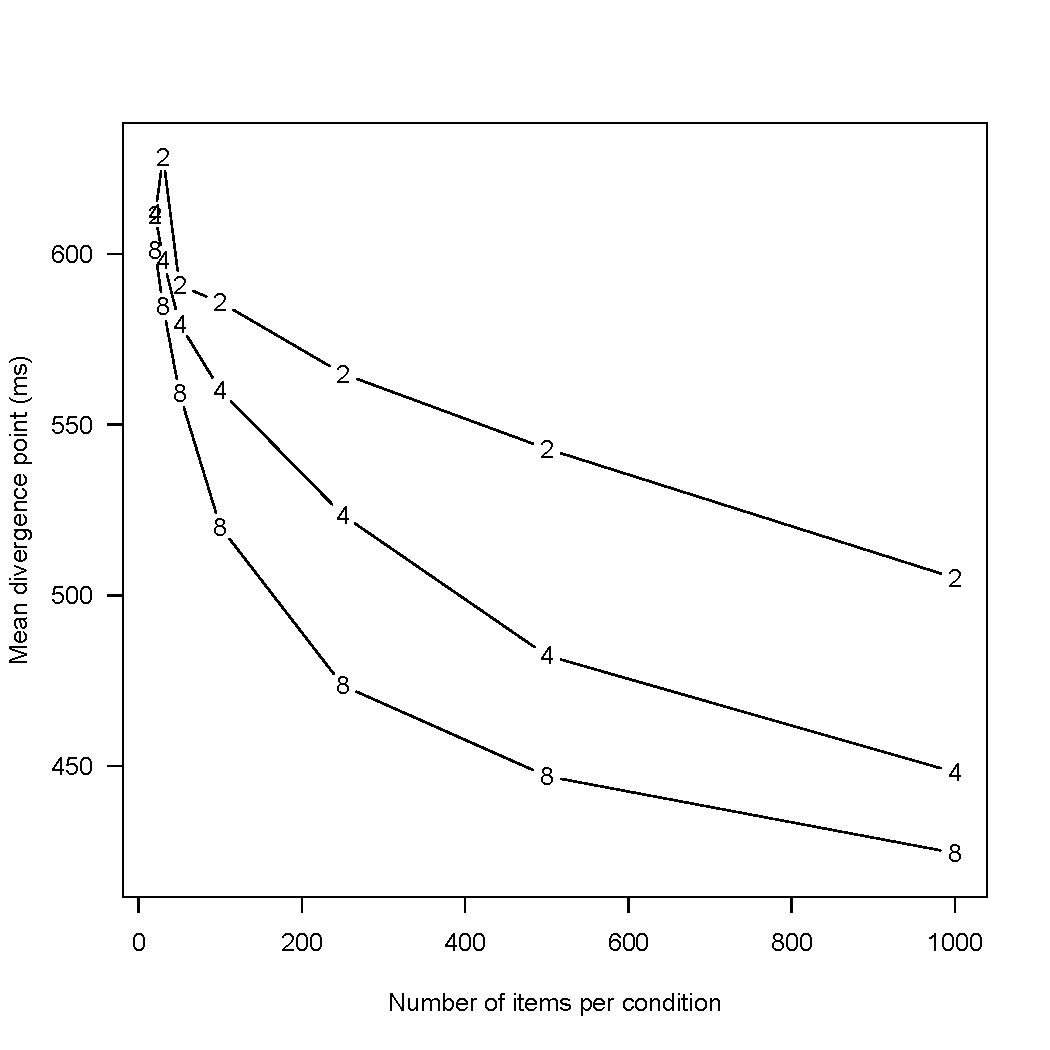
\includegraphics[width=3in]{Figure5.pdf}
	\label{fig:sim2}
	\caption{The figure shows average diverge point for simulation 2. }
\end{figure}
  
      In the third simulation, we generated latency data in which the difference between the two conditions was an effect on $\tau$.  The data for the baseline condition was the same as in the previous simulations: it was generated from an ex-Gaussian distribution with $\mu= 541$, $\sigma = 68$, and $\tau = 115$.  We generated data for three simulated experimental conditions by changing $\tau$ to 135, 155 and 195  ($\Delta \tau = 20, 40, 80$). As shown in Figure 2, changes in $\tau$  produce stochastic dominance of the baseline condition and the true divergence point is at the starting point of the distributions.   The results from this simulation are very similar to those from Simulation 2: The estimation of the divergence point is severely biased by the number of trials per condition (n = 20, 30, 50, 100, 250 or 500).   Figure 6 shows the average divergence point for each of the parameter combinations ($\tau$ and $n$) across 1000 simulations.
       
      In sum, the method of estimating divergence points from two latency distributions does not generate false positives beyond the $\alpha$ level stated by the method; but more importantly, when two latency distributions differ, the method provides an answer that is heavily determined by the number of observations per condition.
      
          
\begin{figure}[h] %  figure placement: here, top, bottom, or page
	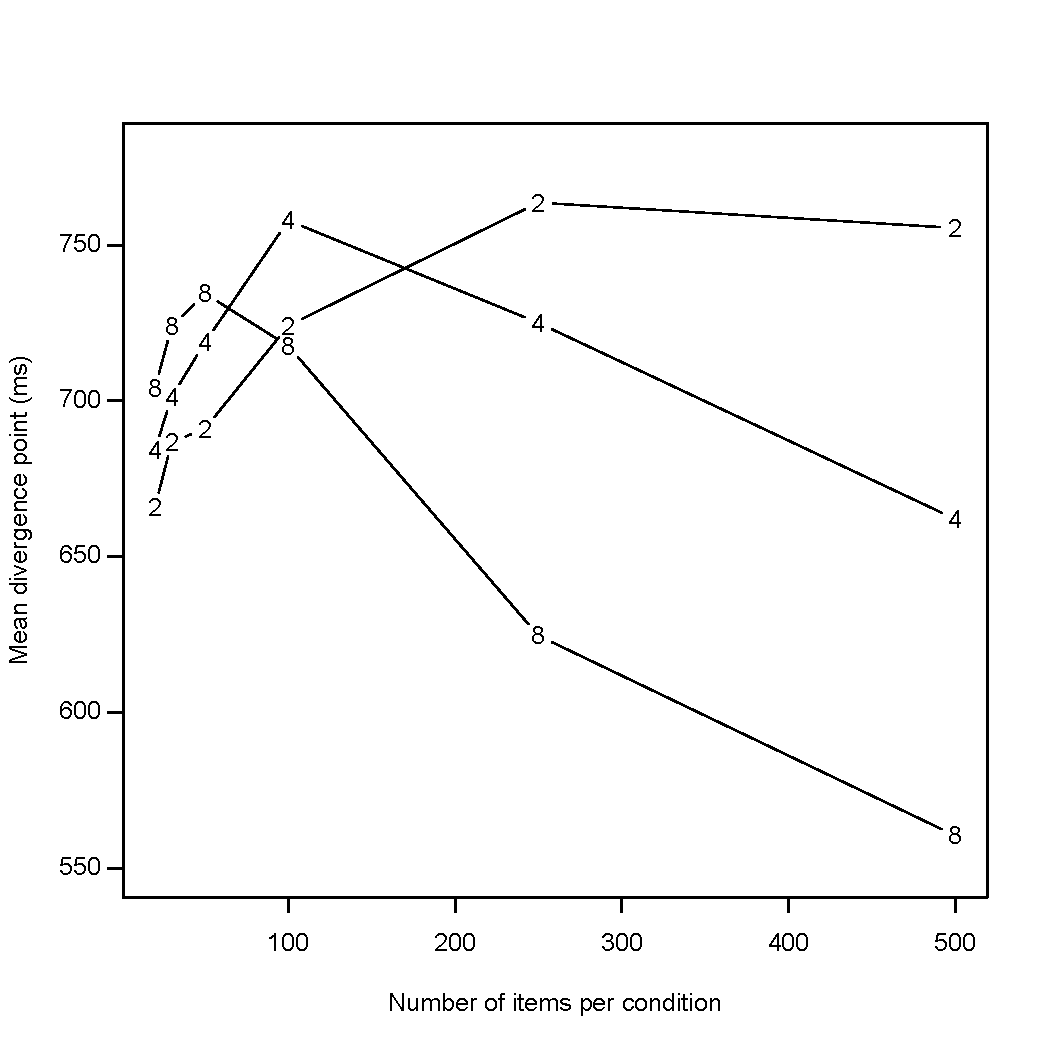
\includegraphics[width=3in]{Figure6.pdf}
	\label{fig:sim3}
	\caption{The figure shows average diverge point for simulation 3. }
\end{figure}


 
            
  
\section{Conclusion}

Although the goals of the divergence point method are worth pursuing, our analysis revealed serious shortcomings on the conceptual foundation of the procedure:  Latency measurements tend to exhibit stochastic dominance between experimental conditions, and hence the divergence point would be at the leading edge of the latency distribution regardless of other distributional differences.  Furthermore, if the method is applied to data, an estimate of the divergence point will be provided by the method. This estimate will be affected mostly by the number of observations.   In short, our exploration of the method forces us to conclude that it is not advisable to utilize it when analyzing latency data.


\section{References}

Ando, E., Matsuki, K., Sheridan, H., \& Jared, D. (2015). The locus of Katakana-English masked phonological priming effects. \emph{Bilingualism: Language and Cognition, 18,} 101-117. DOI: dx.doi.org/10.1017/S1366728914000121


Balota, D. A., \& Yap, M. J. (2011). Moving beyond the mean in studies of mental chronometry the power of response time distributional analyses. \emph{Current Directions in Psychological Science, 20,} 160-166. doi: 10.1177/0963721411408885


Carreiras, M., Armstrong, B.C., Perea, M. \& Frost, R. , ( 2014 ) The What, When, Where, and How of Visual Word Recognition. \emph{Trends in Cognitive Sciences, 18,} 90-98.


Gomez, P., Perea, M., \& Ratcliff, R. (2013). A diffusion model account of masked vs. unmasked priming: Are they qualitatively different? \emph{Journal of Experimental Psychology: Human Perception and Performance, 39,} 1731-1740. DOI: 10.1037/a0032333


Heathcote, A., Popiel, S. J., \& Mewhort, D. J. (1991). Analysis of response time distributions: An example using the Stroop task. \emph{Psychological Bulletin, 109,} 340. DOI: 10.1037/0033-2909.109.2.340


Heathcote, A., Brown, S., Wagenmakers, E. J., \& Eidels, A. (2010). Distribution-free tests of stochastic dominance for small samples. \emph{Journal of Mathematical Psychology, 54,} 454-463. doi:10.1016/j.jmp.2010.06.005

Ratcliff, R. (1978). A theory of memory retrieval. \emph{Psychological Review, 85,} 59-108. doi:10.1037/0033-295X.85.2.59 

Ratcliff, R. (1979). Group reaction time distributions and an analysis of distribution statistics. \emph{Psychological Bulletin, 86,} 446-461. doi: dx.doi.org/10.1037/0033-2909.86.3.446

Reichle, E. D., Pollatsek, A., Fisher, D. L., \& Rayner, K. (1998). Toward a model of eye movement control in reading. \emph{Psychological Review, 105,} 125 -157.

Reingold, E. M., Reichle, E. D., Glaholt, M. G., \& Sheridan, H. (2012). Direct lexical control of eye movements in reading: Evidence from a survival analysis of fixation durations. \emph{Cognitive Psychology, 65,} 177-206.


Reingold, E. M., \& Sheridan, H. (2014). Estimating the divergence point: a novel distributional analysis procedure for determining the onset of the influence of experimental variables. \emph{Frontiers in Psychology, 5,} 1432. doi: 10.3389/fpsyg.2014.01432

Sheridan, H. (2013). The Time-course of Lexical Influences on Fixation Durations during Reading: Evidence from Distributional Analyses. Doctoral Dissertation, University of Toronto. Retrieved from {\texttt https://tspace.library.utoronto.ca/bitstream/1807/35996/6/Sheridan\_Heathe\_201306\_PhD\_thesis.pdf}

Sheridan, H., \& Reingold, E. M. (2013). Distinct stages of word identification during reading: Evidence from eye movements. \emph{Journal of Vision, 13,} 511-511. DOI: 10.1167/13.9.511

Sheridan, H., Rayner, K., \& Reingold, E. M. (2013). Unsegmented text delays word identification: Evidence from a survival analysis of fixation durations. \emph{Visual Cognition, 21,} 38-60. DOI: 10.1080/13506285.2013.767296

Houpt, J. W., \& Townsend J. T. (2010). The statistical properties of the survivor interaction contrast. \emph{Journal of Mathematical Psychology, 54,} 446?453. doi:10.1016/j.jmp.2010.06.006

Houpt, J. W., \&. Townsend, J. T. (2011). An extension of SIC predictions to the Wiener coactive model, \emph{Journal of Mathematical Psychology, 55,}  267-270. doi: dx.doi.org/10.1016/j.jmp.2011.02.002.


Van Zandt, T. (2002). Analysis of response time distributions. In J. T. Wixted (Ed.), \emph{Stevens' Handbook of Experimental Psychology (3rd ed., pp. 461-516)}. San Diego, CA: Academic Press. 


Vincent, S. B. (1912). The function of vibrissae in the behavior of the white rat. \emph{Behavioral Monographs, 1} (Whole No. 5).


\bibliography{bibfile-LDT}

\end{document}
